
\chapter{实验评估}
\label{sec:evaluation}

本章将介绍对\sys{}所进行的实验评估。
首先我们介绍实验设置(\ref{sec:setup}),包括所使用的硬件环境以及选取的模型和数据集。
然后是对\sys{}中提出的模型划分方法的性能评估(\ref{sec:performace})。
为了评估\sys{}中提出的模型划分方法的性能,我们在真实环境下选取了来自不同领域的深度神经网络模型,进行了模型并行化训练。
我们关注模型在不同的划分方法下的训练速度,训练速度越快,模型划分的效果越好。
接着为了验证\sys{}中的模型划分方法不会影响原始模型的收敛性,我们设计了训练收敛性验证实验(\ref{sec:convergence})。
我们会在每个实验中介绍实验的细节和结果,并且对结果进行分析。
最后我们对本章内容进行小结(\ref{sec:evaluation-summary})。

\begin{table}[!htbp]
	\centering
	\caption{服务器配置}
	\label{table:setup}
    \begin{tabularx}{0.9\linewidth}{ p{2.0cm} p{6.8cm} X}
        \toprule
        \textbf{配置项} & \textbf{型号} & \textbf{规格} \\
        \midrule
        GPU & Nvidia® TITAN RTX 24GB & 5 \\
        \midrule
        CPU & Intel® Xeon Gold 5118 @ 2.30GHz & 2 \\
        \midrule
        内存 & Samsung M393A4K40BB2-CTD  & 32GB $\times$ 12 \\
        \midrule
        操作系统 & Ubuntu & 4.15.0-88-generic \\
        \midrule
        \multirow{3}*{软件依赖} & PyTorch & 1.8.1 \\
        \cmidrule{2-3}
        & PICOS & 2.4.11 \\
        \cmidrule{2-3}
        & Gurobi & v10.0.0rc2 \\
        \bottomrule
    \end{tabularx}
\end{table}
\section{实验设置}
\label{sec:setup}
\subsection{硬件环境}
\label{sec:hardware}
\begin{table}[h!] % just use this specifier if really needed.
    \centering
    \caption{设备之间的通信拓扑}\label{table:topo}
    \begin{threeparttable}
    \begin{tabular}{ |p{1.5cm}| p{1.5cm}| p{1.5cm}| p{1.5cm}| p{1.5cm}| p{1.5cm}| }
        \hline
        & \textbf{GPU-0} & \textbf{GPU-1}& \textbf{GPU-2}& \textbf{GPU-3}& \textbf{GPU-4} \\
        \hline
        \textbf{GPU-0} & \texttt{X} & \texttt{PIX} & \texttt{NODE}&  \texttt{NODE}& \texttt{NODE} \\
        \hline
        \textbf{GPU-1} & \texttt{PIX} & \texttt{X} & \texttt{NODE} & \texttt{NODE} & \texttt{NODE} \\
        \hline
        \textbf{GPU-2} & \texttt{NODE} & \texttt{NODE} & \texttt{X} & \texttt{PIX} & \texttt{PIX} \\
        \hline
        \textbf{GPU-3} & \texttt{NODE}& \texttt{NODE} & \texttt{PIX} & \texttt{X} & \texttt{PIX} \\
        \hline
        \textbf{GPU-4} & \texttt{NODE}& \texttt{NODE} & \texttt{PIX}& \texttt{PIX} & \texttt{X}\\
        \hline
    \end{tabular}
    \begin{tablenotes}
        \item[1] \texttt{X}: 设备本身。
        \item[2] \texttt{PIX}: 设备之间通过单个PCIe switch连接。
        \item[3] \texttt{NODE}: 设备之间通过PCIe Host Bridge 在同一个NUMA节点内连接。
    \end{tablenotes}
    \end{threeparttable}
\end{table}

\begin{figure}[h]
	\centering
	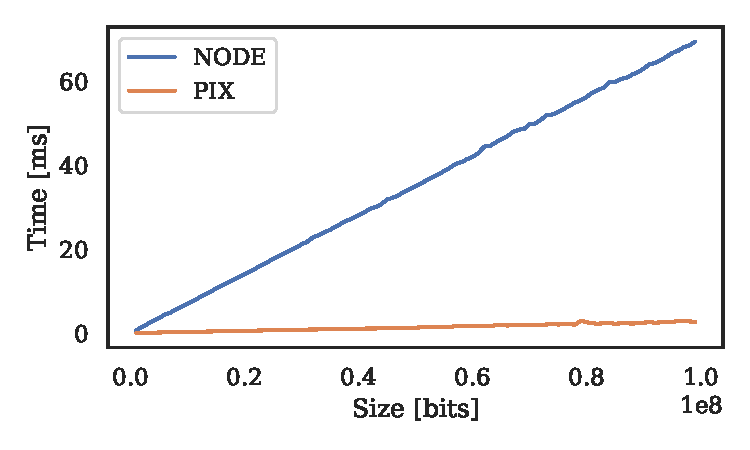
\includegraphics[width=0.75\textwidth]{./figure/5-evaluation/pix-vs-node.pdf}
	\caption{PCIe Switch和PCIe Bridge的通信速度对比}
	\label{fig:switch-vs-bridge}
\end{figure}

我们在一个服务器上进行实验,该服务器的配置如表\ref{table:setup}所示。
在该服务器上有5个型号相同GPU,每个GPU有24GB的显存,由于服务器上并未安装高性能的专用通信设备(例如NVLink)进行连接,因此GPU设备之间的通信链路是异构的,具体来说,GPU的通信拓扑如表\ref{table:topo}所示。


PCIe(Peripheral Component Interconect Express) 是一种高速串行接口总线标准,用于将各种外部设备(例如显卡,网卡,硬盘等)连接到计算机上。
在服务器上,设备之间连接的方式主要有\texttt{PIX}和\texttt{NODE}两种。
\texttt{PIX}是设备通过PCIe Switch使多个PCIe设备连接在一起。在这种方式下,设备共享同一条PCIe总线,设备与设备之间具有高带宽和高吞吐量的连接。
而在\texttt{NODE}连接方式中,设备所使用的PCIe总线通过PCIe Bridge设备连接到NUMA(Non-Uniform Memory Access)节点内的PCIe总线。由于设备之间不共享PCIe总线,所以设备之间的带宽和吞吐相比于\texttt{PIX}有所降低,但是这种方式由于不共享总线,所以具有更好的可扩展性。
图\ref{fig:switch-vs-bridge} 展示了在我们的实验环境中,\texttt{PIX}和\texttt{NODE}两种连接方式下,设备之间通信的速度对比。
图中横轴表示通信数据量,纵轴表示通信时间。
从图中可以看出,通过\texttt{PIX}方式连接的设备之间具有更高的通信速度,反映出了在真实环境中,设备之间采用不同通信链路进行通信时的速度差距。


\subsection{模型与数据集}
在实验中,我们需要比较不同的模型划分方法对于模型训练速度的影响。
为了说明\sys{}中的模型划分方法具有通用性,我们分别从图像分类领域和图像分割领域选择数据集和模型进行实验。

\noindent\textbf{数据集}:在数据集方面,我们选择来自图像分类领域的ImageNet数据集\upcite{imagenet} 和来自图像分割领域的VOC2012数据集\upcite{voc2012}。
\begin{itemize}
	\item ImageNet: 该数据集包含了来自1000个类别的超过120万张高分辨率图像,用于训练和评估图像分类模型。数据集中的每个图像都被进行了标记。ImageNet在图像分类竞赛和图像分类的研究论文中作为基准数据集被广泛使用,因此我们选取ImageNet作为我们的实验数据集之一。
	\item VOC2012: VOC2012是用于目标检测和图像分割领域的数据集,包含来自11500个来自20个不同类别的对象的图像,如人、汽车、动物等。图像中的每个对象都带有一个指定对象在图像中范围的边界框和一个指示对象类别的标签。VOC2012被广泛应用为目标检测和图像分割领域的基准数据集,我们选取VOC2012作为我们的实验数据集之一。
\end{itemize}

\noindent\textbf{模型}: 在模型方面,我们在图像分类模型和图像分割模型中各选择两个大模型进行实验。在图像分类模型中,我们选择AmoebaNet-D\upcite{amoebanet} 和 Wide ResNet-152\upcite{wide}。在图像分割模型中,我们选择了U-Net\upcite{unet} 和DeepLab-V3\upcite{deeplabv3}。
\begin{itemize}
	\item AmoebaNet-D: AmoebaNet-D是AmoebaNet卷积神经网络架构的一种。它使用神经结构搜索算法(Neural Architecture Search, NAS)\upcite{nas} 设计,该算法可以根据给定任务自动搜索合适的网络结构。AmoebaNet-D的特点是具有大量的卷积层和复杂的模型结构,这使其可以学习到复杂的特征,因此AmoebaNet-D在图像分类任务上取得了很好的性能。
	\item Wide ResNet-152: 残差网络(Residual Network)是一种使用残差连接的深度神经网络,ResNet-152\upcite{resnet} 是残差网络的一种,它有152层,包括卷积、池化和全连接的组合。在相关研究\upcite{wide}中,研究者将ResNet中的卷积算子的通道数扩大后发现模型的性能得到了提高。我们在实验中将通道数ResNet-152的通道数扩大2倍,作为我们的待测模型。
	\item U-Net: U-Net是一种用于图像分割任务的卷积神经网络架构,其架构中包括一个对图像进行下采样的编码器和一个对图像进行上采样的解码器,通过采样可以让U-Net捕捉到图像在不同层次下的特征,目前U-Net已经被广泛应用于图像分割任务中。
	\item DeepLab-V3: DeepLab-V3是一种基于编码器/解码器结构的图像分割模型,通常,DeepLab-V3中,使用ResNet等其他卷积神经网络作为编码器,提取图像的特征,然后使用解码器从特征中生成分割结果。我们在实验中使用 Wide ResNet-152作为DeepLab-V3的编码器。
\end{itemize}
表\ref{table:model} 展示了我们所选用的模型在输入图片为$224\times 224$分辨率下,数据批大小为128时的内存需求,从表中可以看出,这些模型的内存需求已经远远超出我们的实验环境中的单个设备的内存容量(24GB)。

\begin{table}[h!] % just use this specifier if really needed.
    \centering
    \caption{模型内存需求}\label{table:model}
    \begin{tabularx}{0.86\linewidth}{ p{3.5cm} p{3.5cm} X  }
        \toprule 
        \textbf{模型名称} & \textbf{计算图节点数目} & \textbf{内存需求(MB)} \\
        \midrule 
        AmoebeNet-D & 784 & 117756.06 \\
        Wide ResNet-152 & 388 & 115179.77 \\
        U-Net & 134 & 50121.92 \\
        DeepLab-V3 & 417 & 168094.43 \\
        \bottomrule
    \end{tabularx}
\end{table}


\section{训练性能验证}
\label{sec:performace}
\subsection{对比方法}
为了验证\sys{}对于使用模型并行化对大模型进行训练的效果,我们引入了其他四种方法和\sys{}进行对比。
\begin{align}
	& \text{min} & & \mathit{Makespan} \label{eq:p-target-2} & \\
	& \text{s.t.} & & \mathcal{S}_{i}=0 &\Gamma^{-}(i)=0, i\in \mathcal{V} \nonumber\\
	& & & \mathcal{C}_{i} = \mathcal{S}_{i} + \mathit{p}_i & \forall i\in \mathcal{V} \nonumber\\
	& & & \mathit{Makespan} \ge \mathcal{C}_{i} & \forall i\in \mathcal{V}\nonumber\\
	& & & \sum_{p=1}^{m} \mathcal{X}_{i,p}=1, \mathcal{X}_{i,p}\in\{0,1\} & \forall i\in \mathcal{V} \nonumber\\
	& & & \mathit{Commu}_{i,j} = \sum_{p\neq q}\mathcal{X}_{i,p}\mathcal{X}_{j,q}F_{\mathit{commu}}(i,j,p,q) & \forall \left\langle i,j\right\rangle \in \mathcal{E} \nonumber\\
	& & & \mathcal{S}_{j} \ge \mathcal{C}_{i} + \mathit{Commu}_{i,j}&\forall \left\langle i,j\right\rangle \in \mathcal{E} \nonumber
\end{align}

\begin{itemize}
	\item \texttt{m-TOPO}: \texttt{m-TOPO}是Baechi\upcite{baechi}提出的三种模型划分放置算法之一,全称为Memory-Constrained Topological Sort Placer。该算法的思路是对计算图中所有的节点进行拓扑排序,然后依次放置在当前设备上,直到达到当前设备的内存容量限制,再转向下一个设备继续放置。Baechi中将设备的内存容量限制设置为$\sum_{i\in\{n\}}d_i / m + \mathrm{max}_{i\in\{n\}} d_i$,其中$m$为设备数目,$d_i$为节点$i$的内存用量。通过这种方式,可以控制每个设备具有近似的内存用量。
	\item \texttt{m-ETF}: \texttt{m-ETF}是Baechi\upcite{baechi} 中提出的另一种模型划分放置算法,全称为Memory-Constrained Earliest Task First。该算法在最早任务优先调度算法\upcite{etf} 的基础上改进得到。该算法维护一个队列,队列中放置着所有的节点和设备的组合$(i,p)$,其中$i$表示节点,$p$表示设备。$(i,p)$按照最早可调度时间升序排列,最早可调度时间的计算按照式\ref{eq:etf}得到。
	\begin{equation}
		\label{eq:etf}
		\mathrm{ETF}(i,p) = \max\left[\mathit{free(p)}, \max_{i\in \Gamma^- (j)}(s_i+k_i+c_{ij}x_{ip}) \right]
	\end{equation}
	式\ref{eq:etf}中,节点$i$在设备$p$上的最早可调度时间为设备$p$的空闲时间和节点$i$的所有前驱节点$j$完成用时中的最大值。
	\texttt{m-ETF}依次从队列中取出当前可调度时间最小的组合$(i,p)$,如果设备$p$的剩余内存可以放置节点$i$,则将节点$i$放置到设备$p$,并更新设备$p$的空闲时间$\mathit{free}(p)$和$i$的所有后继的最早可调度时间。重复这个过程直到所有节点都被调度。

	\item \texttt{m-SCT}: 该算法是在经典的调度算法最小通信时间调度\upcite{sct}上改进得到。在\texttt{m-SCT}中,首先通过整数线性规划(Integer Linear Program)以最小化整体完成时间为目标,为每个节点寻找一个最优子节点,并优先将节点和其最优子节点放置在同一个设备上。
	\item \texttt{Pesto}: 同时,我们也对比了\texttt{Pesto}和我们的方法,由\texttt{Pesto}的原始约束优化问题(\ref{sec:pesto})只能适用于设备数目为2的情况,我们对其进行了扩展。我们采用和\sys{}类似的方法,使用多个指示变量来表示节点在设备上的放置。修改后的\texttt{Pesto}的约束优化问题定义为式\ref{eq:p-target-2}。
\end{itemize}







% \section{实验结果}
% 本节将介绍\sys{}和其他模型划分方法在性能上的对比(\ref{sec:performace})。此外,为了验证\sys{}并不会影响模型的收敛性,还将在\ref{sec:convergence}中对模型训练的收敛性进行验证,最后会在\ref{sec:partition-result}展示模型划分的效果图。

\subsection{实验结果及分析}


\begin{figure}[ht]
	\centering
	\begin{subfigure}[b]{0.45\textwidth}
	  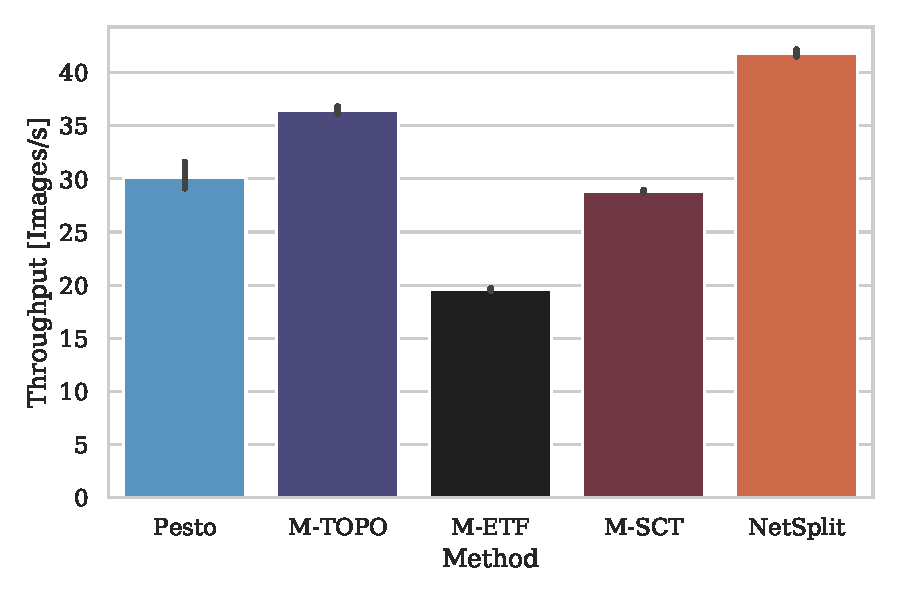
\includegraphics[width=\textwidth]{./figure/5-evaluation/result-amoebanetd.pdf}
	  \caption{AmoebaNet-D}
	\end{subfigure}
	\quad
	\begin{subfigure}[b]{0.45\textwidth}
	  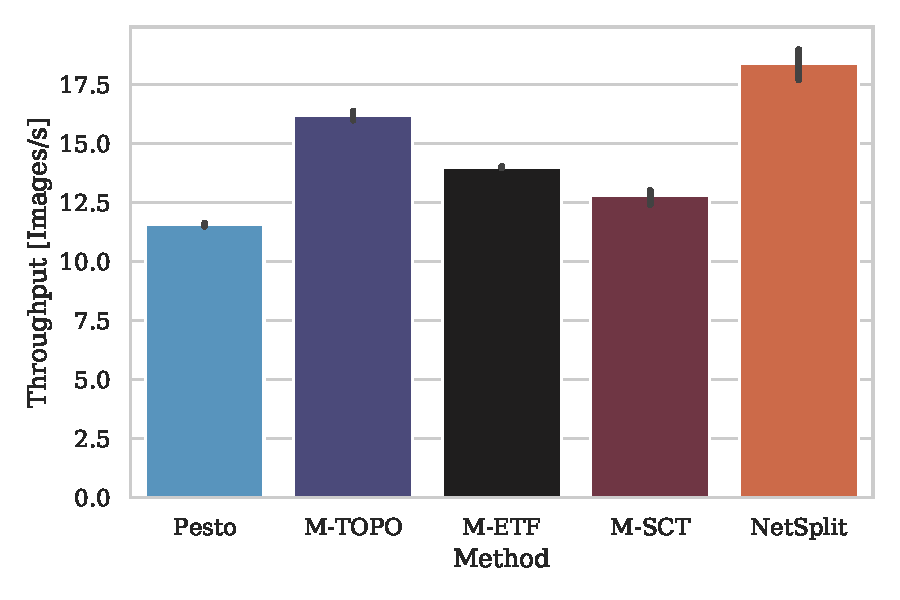
\includegraphics[width=\textwidth]{./figure/5-evaluation/result-deeplabv3.pdf}
	  \caption{DeepLab-V3}
	\end{subfigure}
	\vskip\baselineskip
	\begin{subfigure}[b]{0.45\textwidth}
	  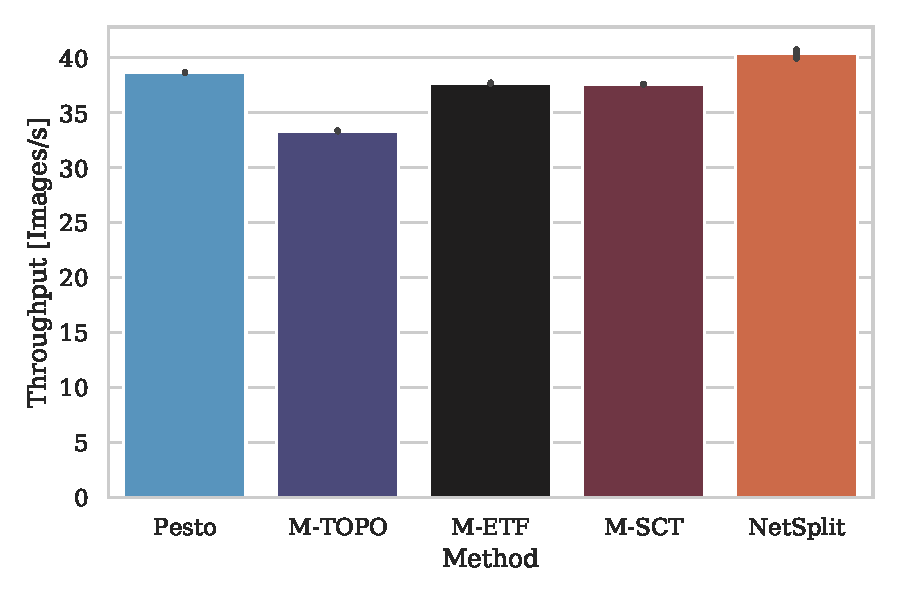
\includegraphics[width=\textwidth]{./figure/5-evaluation/result-unet.pdf}
	  \caption{U-Net}
	\end{subfigure}
	\quad
	\begin{subfigure}[b]{0.45\textwidth}
	  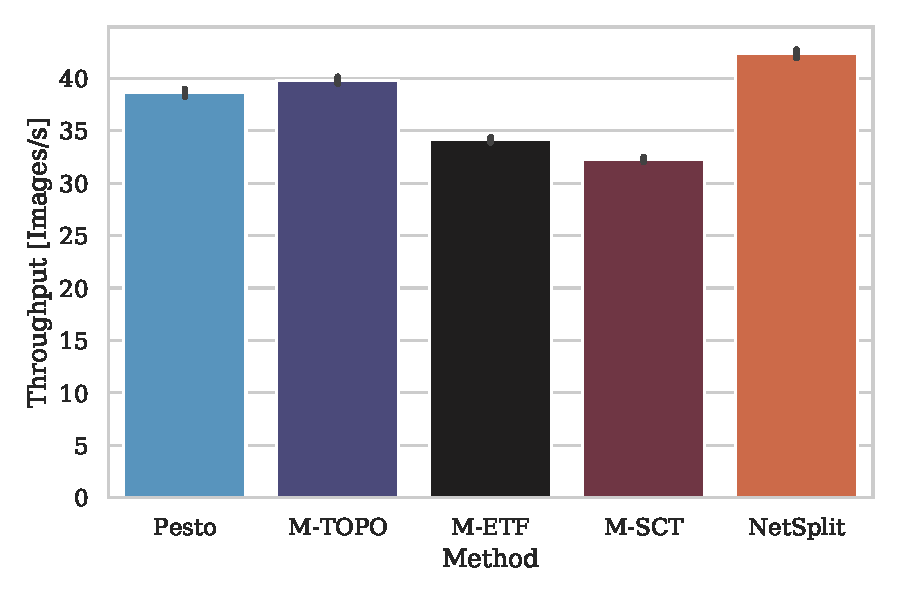
\includegraphics[width=\textwidth]{./figure/5-evaluation/result-wide-resnet152.pdf}
	  \caption{Wide ResNet-152}
	\end{subfigure}
	\caption{\sys{}和其他模型划分方法在4个不同模型上的对比}
	\label{fig:result}
\end{figure}

我们选择\ref{sec:setup}中提到的模型和数据集进行训练,并在训练过程中采集100个数据批的训练用时,计算出每个数据批的平均用时和数据吞吐量。
我们选用3个GPU对每个模型进行训练,其中GPU-0和GPU-1以及GPU-2之间通过\texttt{NODE}的方式进行连接,GPU-1和GPU-2之间通过\texttt{PIX}的方式进行连接。
对于每一个模型,具体的配置为:
\begin{itemize}
	\item AmoebaNet-D: 我们使用18层的AmoebaNet-D,在ImageNet数据集上进行训练,数据批大小设置为64。
	\item Wide ResNet-152: 使用ImageNet数据集进行训练,数据批大小设置为64。
	\item U-Net: 使用VOC2012数据集进行训练,数据批大小设置为128。
	\item DeepLab-V3: 使用VOC2012数据集进行训练,数据批大小设置为48。
\end{itemize}

图\ref{fig:result} 展示了在相同的硬件环境下,在不同模型上使用不同的模型划分方法进行模型并行化训练时数据吞吐量的对比。
从图中可以看出,几种对比方法在不同的模型上表现各有优劣。而相比于几种对比方法,\sys{}在不同的模型上都获得了更高的数据吞吐量,可以在单位时间内完成更多的样本数据的训练,因此可以有效的提升训练速度。

\begin{table}
    \centering
    \caption{性能比较}\label{table:performance}
    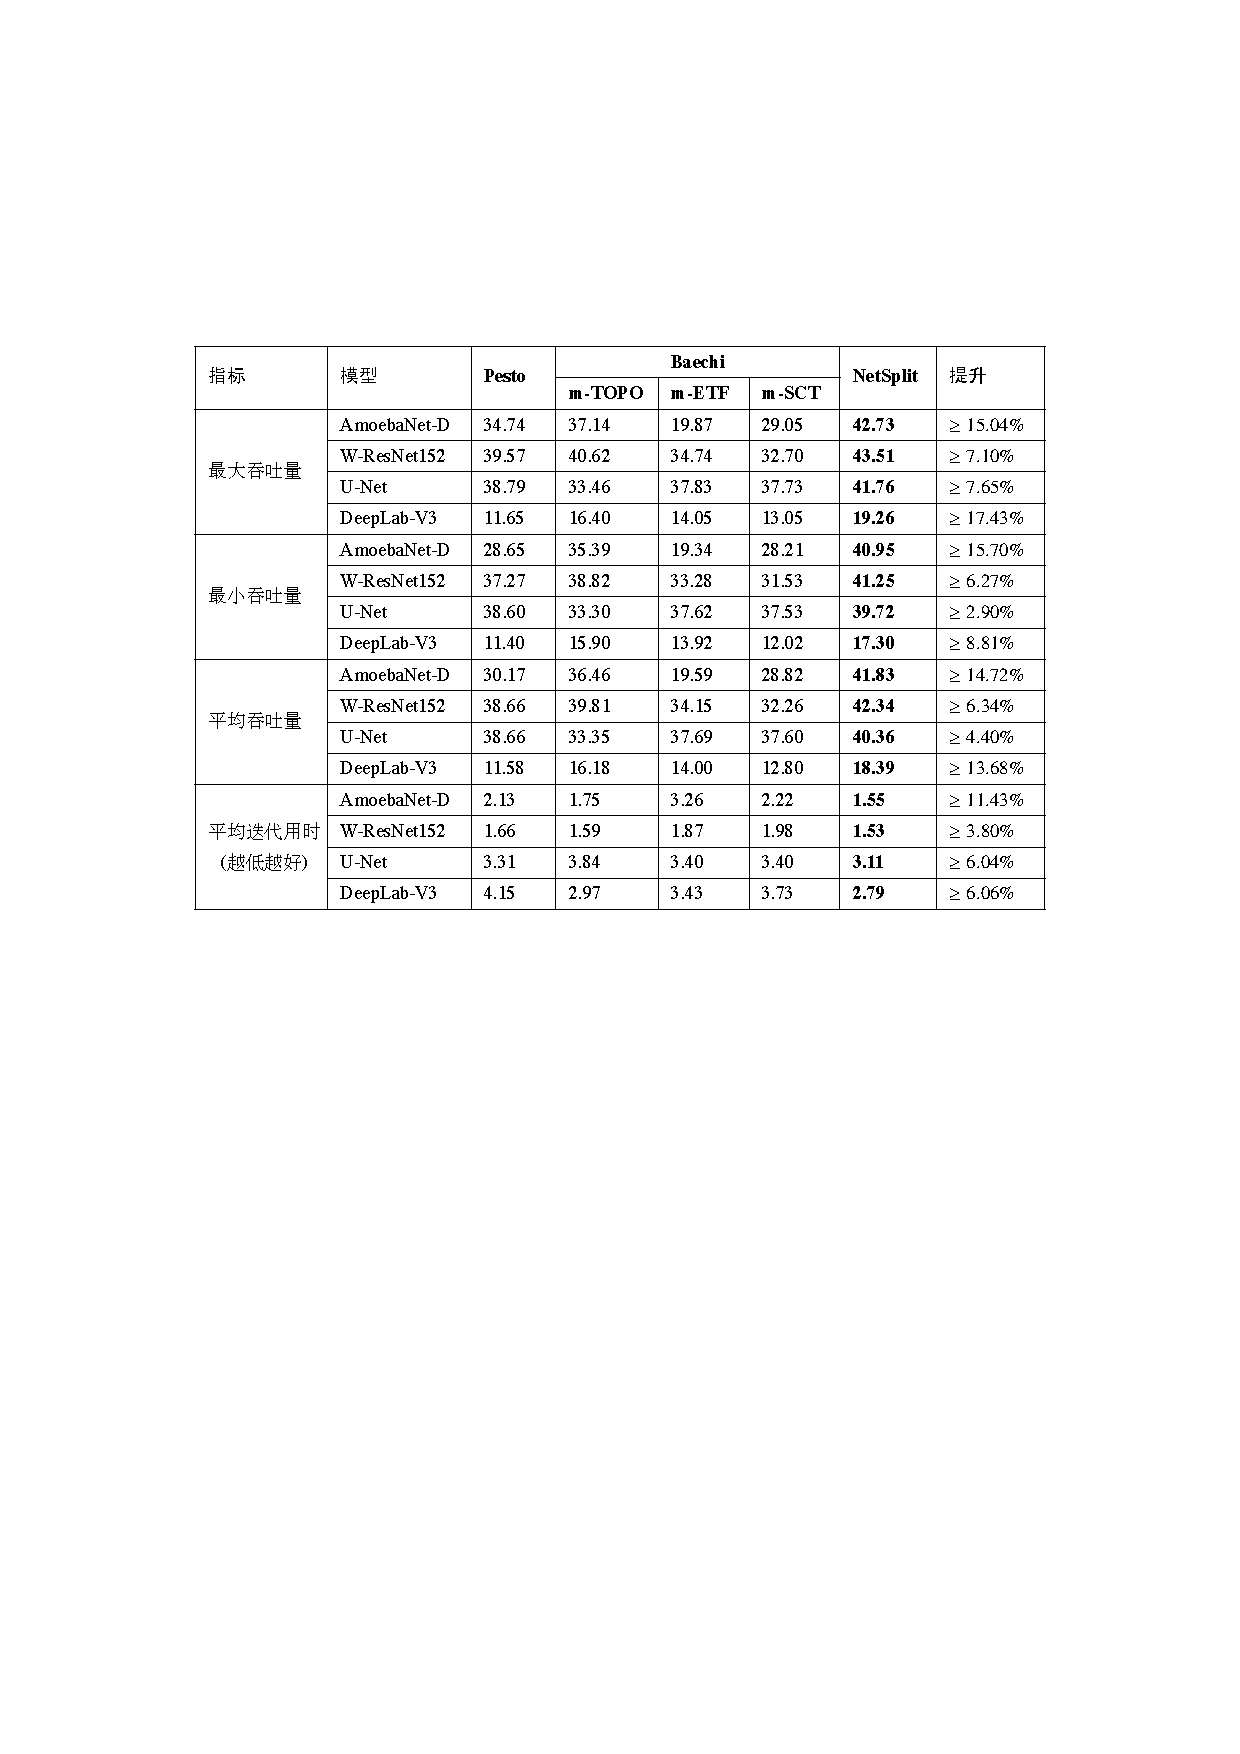
\includegraphics[width=0.98\textwidth]{figure/5-evaluation/performance-table.pdf}
\end{table}

% \begin{table}[h!] % just use this specifier if really needed.
%     \centering
%     \caption{性能比较}\label{table:performance}
%     \tiny
%     \begin{tabular}{ |p{1.8cm} |p{2.0cm} |p{1.0cm} |p{1.3cm} |p{1.1cm} |p{1.1cm} |p{1.2cm} |p{1.4cm}| }
%         \hline
%         \multirow{2}{*}{\textbf{指标}} & \multirow{2}{*}{\textbf{模型}} & \multirow{2}{*}{\textbf{Pesto}} & \multicolumn{3}{c|}{\textbf{Baechi}} & \multirow{2}{*}{\textbf{NetSplit}}  & \multirow{2}{*}{\textbf{提升}}  \\ 
%         \cline{4-6} 
%         & & &\textbf{m-TOPO} & \textbf{m-ETF} & \textbf{m-SCT} & &\\  
%         \hline
%         \multirow{4}{*}{最大吞吐量} & AmoebaNet-D  &  34.74 & 37.14 & 19.87 & 29.05 & \textbf{42.73} & $\ge 15.04\%$ \\
%                                   \cline{2-8}
%                                   & W-ResNet152 &39.57 & 40.62 & 34.74 & 32.70 & \textbf{43.51} & $\ge 7.10\%$ \\
%                                   \cline{2-8}
%                                   & U-Net          &38.79 & 33.46 & 37.83 & 37.73 & \textbf{41.76} & $\ge 7.65\%$ \\
%                                   \cline{2-8}
%                                   & DeepLab-V3    &11.65 & 16.40 & 14.05 & 13.05 & \textbf{19.26} & $\ge 17.43\%$ \\
%         \hline
%         \multirow{4}{*}{最小吞吐量} & AmoebaNet-D  &  28.65 & 35.39 & 19.34 & 28.21 & \textbf{40.95} & $\ge 15.70\%$ \\
%                                   \cline{2-8}
%                                   & W-ResNet152 &37.27 & 38.82 & 33.28 & 31.53 & \textbf{41.25} & $\ge 6.27\%$ \\
%                                   \cline{2-8}
%                                   & U-Net          &38.60 & 33.30 & 37.62 & 37.53 & \textbf{39.72} & $\ge 2.90\%$ \\
%                                   \cline{2-8}
%                                   & DeepLab-V3    &11.40 & 15.90 & 13.92 & 12.02 & \textbf{17.30} & $\ge 8.81\%$ \\
%         \hline
%         \multirow{4}{*}{平均吞吐量} & AmoebaNet-D  & 30.17 & 36.46 & 19.59 & 28.82 & \textbf{41.83} & $\ge 14.72\%$ \\
%                                   \cline{2-8}
%                                   & W-ResNet152 &38.66 & 39.81 & 34.15 & 32.26 & \textbf{42.34} & $\ge 6.34\%$ \\
%                                   \cline{2-8}
%                                   & U-Net         &38.66 & 33.35 & 37.69 & 37.60 & \textbf{40.36} & $\ge 4.40\%$ \\
%                                   \cline{2-8}
%                                   & DeepLab-V3     &11.58 & 16.18 & 14.00 & 12.80 & \textbf{18.39} & $\ge 13.68\%$ \\
%         \hline
%         \multirow{4}{*}{\makecell{平均迭代用时\\(越低越好)}} & AmoebaNet-D    &2.13& 1.75& 3.26& 2.22&  \textbf{1.55} &  $\ge 11.43\%$\\
%                                                          \cline{2-8}
%                                                         & W-ResNet152 & 1.66& 1.59& 1.87& 1.98& \textbf{1.53} & $\ge 3.80\%$\\
%                                                          \cline{2-8}
%                                                         & U-Net          & 3.31& 3.84& 3.40& 3.40& \textbf{3.11} & $\ge 6.04\%$ \\
%                                                          \cline{2-8}
%                                                         & DeepLab-V3     & 4.15& 2.97& 3.43& 3.73& \textbf{2.79} & $\ge 6.06\%$\\
%         \hline
%     \end{tabular}
% \end{table}


% \begin{table}[h!] % just use this specifier if really needed.
%     \centering
%     \caption{性能比较}\label{table:performance}
%     \tiny
%     \begin{tabularx}{\linewidth}{ p{1.4cm} p{1.7cm} p{1.4cm} p{1.4cm} p{1.4cm} p{1.4cm} p{1.4cm} p{1.2cm}}
%         \toprule 
%         \multirow{2}{*}{\textbf{指标}} & \multirow{2}{*}{\textbf{模型}} & \multirow{2}{*}{\textbf{Pesto}} & \multicolumn{3}{c}{\textbf{Baechi}} & \multirow{2}{*}{\textbf{NetSplit}}  & \multirow{2}{*}{提升}\\ 
%         \cmidrule{4-6} 
%         & & &\textbf{m-TOPO} & \textbf{m-ETF} & \textbf{m-SCT} & \\  
%         \midrule
%         \multirow{4}{*}{最大吞吐量} & AmoebaNet-D    & & & & & & \\
%                                   \cmidrule{2-8}
%                                   & W-ResNet152 & & & & & & \\
%                                   \cmidrule{2-8}
%                                   & U-Net          & & & & & & \\
%                                   \cmidrule{2-8}
%                                   & DeepLab-V3     & & & & & & \\
%         \midrule
%         \multirow{4}{*}{最小吞吐量} & AmoebaNet-D    & & & & & & \\
%                                   \cmidrule{2-8}
%                                   & W-ResNet152 & & & & & & \\
%                                   \cmidrule{2-8}
%                                   & U-Net          & & & & & & \\
%                                   \cmidrule{2-8}
%                                   & DeepLab-V3     & & & & & & \\
%         \midrule
%         \multirow{4}{*}{平均吞吐量} & AmoebaNet-D    & & & & & & \\
%                                   \cmidrule{2-8}
%                                   & W-ResNet152 & & & & & & \\
%                                   \cmidrule{2-8}
%                                   & U-Net          & & & & & & \\
%                                   \cmidrule{2-8}
%                                   & DeepLab-V3     & & & & & & \\
%         \midrule
%         \multirow{4}{*}{平均迭代用时} & AmoebaNet-D    & & & & & & \\
%                                     \cmidrule{2-8}
%                                     & W-ResNet152 & & & & & & \\
%                                     \cmidrule{2-8}
%                                     & U-Net          & & & & & & \\
%                                     \cmidrule{2-8}
%                                     & DeepLab-V3     & & & & & & \\
%         \bottomrule
%     \end{tabularx}
% \end{table}

表\ref{table:performance}展示了几种不同的模型划分方式下,进行模型并行化训练时的性能比较。
对比表中的数据我们发现,\sys{}和其他的方法相比,在不同的模型和数据集上,可以有效提升平均数据吞吐量$4.4\% \sim 14.72\%$,相应的,平均迭代用时,也就是模型训练每个数据批的时间减少了$3.8\% \sim  11.43\%$。
由于采样误差和训练过程中其他开销(数据预处理,磁盘IO等)的影响,导致平均数据吞吐量的提升和平均迭代用时的减少略有一些差异。
总的来说,相比于其他方法,使用\sys{}进行模型划分,可以有效提升模型并行化的训练效率,提升集群中的硬件资源利用率,缩短训练任务的用时。


在几种被测模型中,对于模型大小更大的AmoebaNet-D和DeepLab-V3,\sys{}的表现最好,相比于其他几种方法,在吞吐量方面有超过$13.68\%$的提升。
而对于模型大小较小的U-Net,\sys{}相比于其他几种方法中表现最好的\texttt{Pesto}来说,提升只有$4.40\%$。
对于AmoeBaNet-D和DeepLab-V3这种计算图中含有大量节点和边的复杂模型,在进行训练时,设备需要进行大量运算来得到反向传播的中间结果。同时由于模型的计算图中有大量的边,导致模型训练过程的实际通信代价较大,因此针对异构通信环境并且在约束优化问题的求解中加入反向传播的\sys{}在这样的复杂模型上表现更好。而没有考虑反向传播用时和异构的通信环境的\texttt{Pesto}在面对这样的复杂模型时,性能反而不如一些近似算法。

\subsection{有效性威胁分析}
\label{sec:threat}
% 1. 我们在单个主机的多个设备上进行实验,在这种情况下,p2p通信只发生在设备内部。尽管我们没有将实验扩展到多个主机的多个设备,并且让部分通信发生在网络上,但是这并不会影响建模准确性。因为即使是在单个主机上,设备之间的通信链路也是异构的,从实验结果上,在单机上有效
% 2. 在数据集和模型的选择上,我们选择来自图像领域的模型和数据集,而没有选择如文字、音频和视频等数据集。why? 图像识别有代表性,不同的任务领域的训练模式和特征是一样的,都是迭代式训练。


在实验场景的选择上,在\sys 对于模型训练性能的提升的实验评估中,我们将模型划分到位于单个主机的多个设备上进行训练,此时设备之间的通信只发生在主机的内部。而在真实的模型训练场景下,模型有可能被划分到位于多个主机的多个设备上,这种情况下,部分通信通过主机之间互联的网络进行。因此在单机场景下的实验也许无法反映真实场景下不同方法的性能差距。但是在单个主机上,设备之间的通信链路也是异构的,例如设备之间有可能通过PCIe Switch 连接,也有可能通过PCIE Host Bridge 连接,这种异构性和真实场景下的通信类似,因此,\sys 中对于问题的建模可以用于真实的场景。未来可以尝试更加真实场景下的设备和通信方式。



在数据集和模型的选择上,我们选择了图像领域的模型和数据集作为实验对象,因此,我们尚不清楚我们的框架在其他领域的模型和数据集的效果如何。但由于图像识别是最具有代表性、最被广泛研究的深度学习任务之一,并且我们选择的模型和数据集都是广泛被使用的基准测试,我们相信我们的评估结果在一定程度上是可靠的。我们将在未来工作中增加对文本、音频、视频等领域模型和数据集的评估。


\section{训练收敛性验证}
\label{sec:convergence}
我们设计了训练收敛性实验来验证\sys{}中对模型所进行的转换操作以及模型划分操作不会影响原始模型的性能。

\subsection{对比方法}
\begin{table}[h!] % just use this specifier if really needed.
    \centering
    \caption{收敛性验证实验配置}\label{table:convergence-setup}
    \begin{tabularx}{0.66\linewidth}{ p{3.5cm} X  }
        \toprule 
        \textbf{配置项} & \textbf{配置值}\\
        \midrule 
        模型 & ResNet-152 \\
        数据集 & ImageNet \\
        数据批大小 & 64 \\ 
        设备数目 & 4 \\
        学习率 & 1e-4 \\ 
        优化器 & Adam Optimizer \\
        \bottomrule
    \end{tabularx}
\end{table}

如本文\ref{sec:convertion} 中所述,当用户向\sys{}提交以PyTorch中\texttt{nn.Module}格式定义的模型后,\sys{}会将用户的模型转化成计算图的中间表示,在划分完成后,\sys{}还会将中间表示转化成\texttt{fx.GraphModule}。
在进行第二步转化时,会在模型中根据划分结果插入一些额外的节点,完成跨设备的变量转移。
因此为了验证经过多次转化和修改后的模型是否还和原模型在功能上等价,我们设计了收敛性验证实验。

收敛性验证实验的目的是为了验证\sys{}并不会损害原始模型的性能,我们通过测试使用\sys{}训练转换后的模型和使用数据并行化(Data Parallelism, DP)训练的原始模型的收敛性进行验证。
对于数据并行化,我们使用PyTorch中提供的DistributedDataParallel(DDP)\footnote{\url{https://pytorch.org/docs/stable/notes/ddp.html}} 进行训练。
我们使用的实验配置如表\ref{table:convergence-setup} 所示。


\subsection{实验结果及分析}

图\ref{fig:convergence-all} 展示了模型收敛性的验证结果。
其中,图\ref{fig:convergence-epoch}展示了在两种不同的训练方式下,模型的准确率随着训练轮次(Epoch)变化的情况。
我们一共训练了40个轮次,从图中可以看出,在相同的轮次下,两种训练方式得到的模型的准确率几乎相同。
因此可以得到结论,\sys{}并不会损害原始模型的性能,即不会影响原始模型的收敛性。
此外,图\ref{fig:convergence-time} 展示了模型的准确率随着时间的变化情况。
可以看出,由于\sys{}利用了模型并行化方法,有效提升了大模型训练的效率,相比于数据并行化方法,每一轮所需的训练时间更短,模型随着时间的收敛速度更快。

\begin{figure}[ht]
	\centering
	\begin{subfigure}[b]{0.85\textwidth}
	  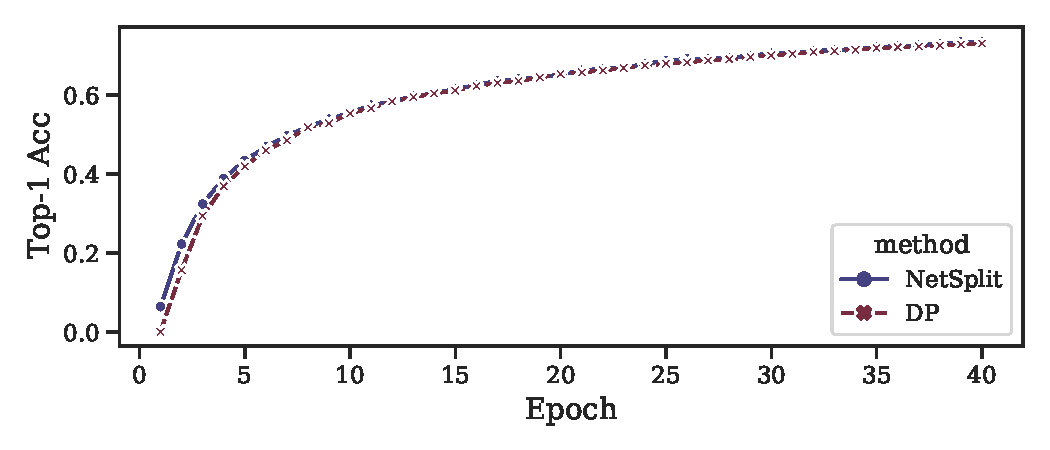
\includegraphics[width=\textwidth]{./figure/5-evaluation/convergence-epoch.pdf}
	  \caption{模型准确率随轮次(Epoch)变化}
	  \label{fig:convergence-epoch}
	\end{subfigure}
	\vskip\baselineskip
	\begin{subfigure}[b]{0.85\textwidth}
	  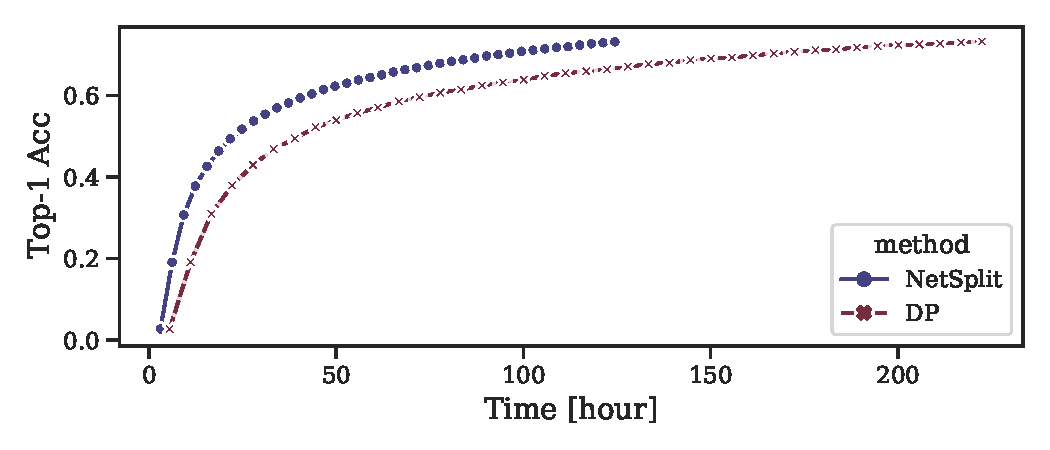
\includegraphics[width=\textwidth]{./figure/5-evaluation/convergence-time.pdf}
	  \caption{模型准确率随时间变化}
	  \label{fig:convergence-time}
	\end{subfigure}
	\caption{收敛性验证}
	\label{fig:convergence-all}
\end{figure}


\section{本章小结}
\label{sec:evaluation-summary}

在本章中,我们详细介绍了针对\sys{}进行的两方面实验,分别是训练性能验证和训练收敛性验证。
训练性能验证实验中,我们将\sys{}和其他的模型并行化方法在真实的模型和数据集上进行训练,通过比较训练时的数据吞吐量来评估训练性能。
实验结果表明,相比于已有方法,\sys{}可以有效提升对大模型进行模型并行化训练的训练效率,缩短训练任务用时。
在训练收敛性验证实验中,我们比较\sys{}和数据并行化的对在相同条件下对同一个模型的训练过程,实验结果表明\sys{}不会影响模型训练过程的收敛性。

下一章(\ref{sec:summary})将总结本文的工作,并展望未来的工作。